\documentclass[]{report}
\usepackage{amsmath, amssymb, graphicx}
\usepackage[margin=0.75in]{geometry}
\graphicspath{{resources/}}


% Title Page
\title{An extension of the formal model for a Library System}
\author{Dominic Rathbone}


\begin{document}
\maketitle

\section{Abstract}
The goal of this document is to extend and refine the functionality of the existing library system by introducing the concept of time to it in accordance with the requirements given in the coursework document.

\section{Class Invariant}
\subsection{Informal statement}
In order to introduce the concept of time into the library system, a type named "DATE" is created and added to the class invariant. At this level, it is used to define a variable "Today" which is the basis of the system's notion of time. The class invariant has also been extended to add reservations and loans by representing each as a subset of the cartesian product of the sets Title and Member. This way, each member of the loan set can be mapped to a "DATE" representing a due date and each member of the reservation subset can be mapped to another "DATE" representing an expiry date. By doing so, the idea of a limited reservation period and permissible loan period is introduced into the system. Modelling the sets this way also gives the system more flexibility as the set of Title and Member is not limited to strictly reservations and loans, thus allowing for further extension. The invariant also contains a new addition to a member, "FinesOwned" which indicates how much money a member owes from overdue loans. In the post-condition, the Loan and Reservation set are initially empty.
\subsection{Formal statement}
\begin{center}
\includegraphics{class_invariant.pdf}
\end{center}
\newpage
\section{Move To Next Day}
\subsection{Informal statement}
In order to introduce the idea of a daily cycle into the system, the "Today" variable set up in the class invariant can be used to derive the next day. To do so, a new event is created that takes in today's date as a parameter. Along with this, to enforce the idea of permissible periods and constraints on reservations into the system, the set of reservations and loans are passed through to check them for expired reservations and overdue loans. In the post-condition, every reservation's expiry date is compared to see if it equal to or after today's date, if it is the reservation is then passed through to the cancel event. Similarly, for each loan, the due date is checked to see if it is equal to today's date or later, if it is, the member is then fined 0.50p. This fine would occur every day until the book is returned.  Today is then incremented by one in order to move to the next day. 
\subsection{Formal statement}
\begin{center}
	\includegraphics{move_to_next_day.pdf}
\end{center}
\newpage
\section{Reserve}
\subsection{Informal statement}
The reserve event has to be updated to add a expiry date when a book is reserved. To do this, it has been updated to take new parameters, "dur" (reservation duration) and "today". To create a new reservation, a rule has been added that means a user must have currently not owe any money in fines to the library. A new pair called r of type Title X Member is then made to represent a new potential reservation. In the post-condition, the new reservation is then added to the set and the expiry date for the new reservation is calculated and linked to the reservation by the "ExpiryDate" function. 
\subsection{Formal statement}
\begin{center}
	\includegraphics[scale=0.75]{reserve.pdf}
\end{center}
\newpage
\section{LoanCopy}
\subsection{Informal statement}
Similar to reserve, the loanCopy event has to be updated to add due dates to new loans taken out. To do this, it is extended to include to new parameters, dur (loan duration) and today. To create a new loan, the member must not owe any fines to the library. A new Title and Member pair is made from the title and member parameters to represent a new potential loan. If the loan is then found to already exist as a reservation, the cancel event is called and the reservation is cancelled. In the post-condition, the due date is calculated by adding the duration to the current date, this is then linked to the new loan by the "DueDate" function.
\subsection{Formal statement}
\begin{center}
	\includegraphics[scale=0.75]{loan_copy.pdf}
\end{center}
\newpage
\section{Cancel}
\subsection{Informal statement}
The cancel event is relatively simple, it takes a reservation, "r", from which the title and member taken and passed through to the simple library system's cancel event. in the post-condition, the reservation is then removed from the set.
\subsection{Formal statement}
\begin{center}
	\includegraphics{cancel.pdf}
\end{center}
\newpage
\section{Return}
\subsection{Informal statement}
Again, similar to the cancel event, the new return event takes a loan as a parameter and uses the title and member with the simple library system's return event. The loan is then removed from the loan set.
\subsection{Formal statement}
\begin{center}
	\includegraphics{return.pdf}
\end{center}
\newpage
\section{ShowDueDate}
\subsection{Informal statement}
This event just takes in a loan and and outputs the due date it has been associated with by the DueDate function.
\subsection{Formal statement}
\begin{center}
	\includegraphics{show_due_date.pdf}
\end{center}
\newpage
\section{ShowExpiryDate}
\subsection{Informal statement}
This event takes in a reservation and and outputs the expiry date it has been associated with by the ExpiryDate function.
\subsection{Formal statement}
\begin{center}
	\includegraphics{show_expiry_date.pdf}
\end{center}
\newpage
\section{Fine}
\subsection{Informal statement}
The idea of a fine was introduced into the system as realistically, not all members would return the book by the date it is due and the system needs to be able to cope with this. This event takes in a member and an amount in the form of a decimal number. It then takes this amount and adds it to the current fine amount owed by the member.
\subsection{Formal statement}
\begin{center}
	\includegraphics{add_fine.pdf}
\end{center}
\newpage
\section{Pay Fine}
\subsection{Informal statement}
This allows the member to pay the fine they currently owed. It takes in a member and amount as parameters. This amount has to be smaller than the or equal to the amount they currently owe, if it's not, the amount is changed to be equal to the current fines. After this, the amount is then subtracted from the current fines.
\subsection{Formal statement}
\begin{center}
	\includegraphics{pay_fine.pdf}
\end{center}
\newpage
\section{Show Fines}
\subsection{Informal statement}
This event takes in a member and and outputs the amount of money they owe via the FinesOwned function.
\subsection{Formal statement}
\begin{center}
	\includegraphics{show_fines.pdf}
\end{center}
\newpage

\end{document}          
